%!TEX program = xelatex
% 完整编译: xelatex -> bibtex -> xelatex -> xelatex
\documentclass[lang=cn,11pt,a4paper]{elegantpaper}
\usepackage{caption}
\usepackage{graphicx}
\usepackage{float}
\usepackage{subfigure} 
\captionsetup{width=0.8\textwidth}
\title{基于多季节模型的中国人民大学东门外主干道路况预测}
\author{王兴睿}
\institute{中国人民大学 统计学院17级一班}

\date{\zhtoday}

\begin{document}

\maketitle

\begin{abstract}
在如今快速发展的城市中,机动车辆给我们的出行带来了便利,但同时也带来了交通拥堵等问题。于是,预测交通路况成为了不论是对城市建设还是个人出行的关键性问题。而在实际分析中,交通路况往往受到双休日、节假日的影响,具有复杂的多重周期性,也同时可能受到突发社会事件比如疫情封城的影响,具有突变的可能性。这些因素都提高了对交通数据的建模的难度。在本次研究中,我以中国人民大学东门外主干道的汽车车速数据为例,建立多季节乘积ARIMA模型ARIMA(1,0,1)(0,0,1)[24](3,0,0)[168]以及多季节Holt-Winters指数平滑模型拟合数据,并预测之后两周内的交通路况变化。之后分别从预测正确率、残差白噪声检验评价两种方法的差异性。比较不同模型的结果,发现多季节Holt-Winters指数平滑模型有更好的预测准确率,但从残差的角度看,多季节ARIMA模型残差自相关程度更小,对原序列的规律性信息提取的更好。另外,也尝试用ARCH(2)模型
对残差进行进一步拟合,结合MSARIMA的结果建立MSARIMA-ARCH模型以达到更好的拟合效果。\href{https://github.com/XingruiWang/ruc_traffic_prediction}{项目
Github地址}
\keywords{交通路况预测,多季节ARIMA模型,双季节Holt-Winters指数平滑}
\end{abstract}

\section{背景介绍}
交通预测是建立智能交通系统(Intelligent Transport System)的重要部分,在个人出行路线智能规划、智能驾驶路线分配以及城市交通系统建设都有关键的意义~\cite{its}。预测交通路况可以帮助减少交通堵塞,提高人们出行效率。对于一些大城市比如北京来说,想要预测出某一条路段未来几小时或者几天内的交通情况无疑是关键而具有挑战的。由于交通数据受到多种因素的影响,比如时间因素如上下班高峰期、节假日、双休日等因素;也有突发社会状况,比如疫情防控期间限制出行、雾霾严重期间汽车限号、举办演唱会或大型活动等事件;也包括空间因素比如道路结构,以及周边道路的路况信息~\cite{bbliaojqZhangKDD18deep}。

在交通预测中,挖掘出数据的时间属性信息是最为重要的。从生活经验来看,交通数据的随时间的变化具有一定的周期性。从每天的规律来看,周内的早上八点和下午六点是每天的上下班高峰期,车流量剧增,很多路段都会发生堵塞现象。从一周来看,很多人愿意在周六选择外出游玩,所以周六往往是一周内路况最差的一天;从更长的周期来看,每逢重大节假日,如五一劳动节、清明节、十一国庆节、新年等等,刚放假和假期快结束的几天正是人们的出城和返城高峰,出行规律也会与往日有很大的差别。

周期性的时间序列可以采用不同方式进行建模。确定性因素分解是一种被广泛运用到具有周期性和趋势性的时间序列建模之中的一种方法,可以将原始数据分解为趋势项、周期项、随机波动项。结合ARIMA模型它们各自的规律以及之间的关系进行进行拟合,可以建立季节ARIMA模型。另外还有指数平滑方法,它将原始序列平滑处理,排除随机波动的干扰,提取出序列的平滑信息、趋势信息、季节信息,拟合历史数据,预测未来数据。

不同建模方法并没有绝对的优劣性[...],所以这篇文章中,我主要采用了(1)多季节的ARIMA模型;(2)多季节的指数平滑模型,也就是双季节Holt-Winters指数平滑模型。并以中国人民大学东门外的主干道车速数据为例,比较不同方法在预测结果上准确率的不同。以下我会从相关研究工作、模型介绍、实验结果、总结和讨论这四个部分进行详细介绍。

\section{相关工作}
交通预测是构建智慧城市、智能交通系统以及个人规划出行的关键。在以往的交通预测方法中,人们主要采用的是非参数和参数两种方法。非参数方法的代表是近年来较为流行的循环神经网络LSTM模型~\cite{ma2015long},具有计算速度,建模灵活的方式,但是解释性较低。参数方法主要有ARIMA模型~\cite{zhang2011data}、平滑模型等。和非参数模型相比,参数模型的系数更具有实际意义,所以模型更能挖掘出时间序列规律性也更加具有解释性。结合交通数据普遍存在的多周期、无明显趋势的特征,可以使用确定性因素分解,结合残差自回归,用不同的参数模型拟合不同周期的季节项和随机波动项\cite{8892991}。或者利用各项之间的关系,建立加法季节ARIMA模型和乘法季节ARIMA模型。多季节ARIMA模型,用来拟合如交通数据的可能同时具有日周期、周周期、月周期、年周期的复杂周期序列~\cite{box2011time}~\cite{taylor2006comparison}~\cite{tran2015multiplicative}。除此之外,也可以用指数平滑法对周期性序列进行建模~\cite{ord1997estimation}。Holt-Winters三参数指数平滑可以处理具有趋势和季节项的序列的时间序列。对于多周期性时间序列,Taylor提出了双季节指数Holt-Winters指数平滑方法(Double Seasonal Holt-Winters exponential smoothing method,简称DSHW
指数平滑法)~\cite{ord1997estimation},在Holt-Winters指数平滑法的基础上,再添加一个新的季节项,用来提取序列中短期周期和长期周期。这种方法也被广泛运用到包括交通预测之内的多周期时间序列预测的问题中~\cite{ord1997estimation}~\cite{shahin2017using}~\cite{gould2008forecasting}。

\section{模型}
\subsection{MSARIMA 多季节ARIMA模型}
一种常见的对季节模型的建立方式是季节SARIMA模型(Seasonal ARIMA)~\cite{box2011time}。根据季节效应提取的方式不同,可以分为加法模型和乘积模型。乘积模型可以提取出季节效应、长期趋势效应、随机波动效应各自的特征以及它们之间交互影响特征,已经成为了处理较为复杂的周期性时间序列的经典方法。

对于含有多个季节效应的中心化时间序列,乘积季节ARIMA模型可以写成如下形式

\begin{equation}
\nabla^d\nabla_{S_1}^{D_1}\ldots\nabla_{S_k}^{D_k}x_t=\frac{\Theta(B)\Theta_{S_1}(B)\ldots\Theta_{S_k}(B)}{\Phi(B)\Phi_{S_1}(B)\ldots\Phi_{S_k}(B)}\varepsilon_t
\end{equation}

其中$x_t$表示在时刻$t$的原观察序列值,$S_1,S_2,\ldots,S_k$表示原序列具有的$k$个不同的时间周期长度,$B$表示延迟因子;$\nabla$表示差分符号,$\nabla_{S_k}^{D_k}$表示进行$D_K$阶的$S_k$步差分,$\varepsilon$表示时间$t$的误差项。$\Theta(B),\Theta_{S_k}(B),\Phi(B),\Phi_{S_k}(B)$分别是$q,Qk,p,Pk$次多项式。MSARIMA模型可以简记为$\mathrm{ARIMA}(p,d,q)\times(P_1,D_1,Q_1)_{S_1}\ldots(P_k,D_k,Q_k)_{S_k}$

特别的,对于双周期ARIMA模型,即令$k=2$,ARIMA模型可以记为$\mathrm{ARIMA}(p,d,q)\times(P_1,D_1,Q_1)_{S_1}\times(P_2,D_2,Q_2)_{S_2}$。

\subsection{双季节Holt-winters指数平滑模型}
双季节Holt-Winters指数平滑(DSHW)是Taylor在预测用电需求时,在Holt-winters三参数指数平滑模型的基础上,构造出来的适用于两周期时间序列的指数平滑模型~\cite{taylor2006comparison}。对于要进行指数平滑的序列${x_t}$,既含有趋势项,也含有两个季节项。记$a_t$为该序列的水平部分,$b_t$为该序列的趋势部分,$s_t,r_t$是该序列的两个季节因子,季节长度分别为$\pi_1,\pi_2$。对于乘法模型,DSHW指数平滑的构造如下:

\begin{equation}
\begin{aligned}
a_t&=\alpha(x_t/s_tr_t)+(1-\alpha)(a_{t-1}+b_{t-1})\\
b_t&=\beta(a_t-a_{t-\Pi_1})+(1-\beta)b_{t-1}\\
s_t&=\gamma(x_t/a_tr_t)+(1-\gamma)s_{t-\pi_1}\\
r_t&=\delta(x_t/a_ts_t)+(1-\delta)r_{t-\pi_1}\\
\end{aligned}
\end{equation}


\section{实验}
\subsection{数据集}
\textbf{Q-Traffic 数据集}:\href{https://ai.baidu.com/broad/introduction?dataset=traffic}{Q-Traffic}是由百度大脑收集的大规模的交通预测数据集~\cite{bbliaojqZhangKDD18deep}。数据集包括Traffic Speed数据集、Road Network数据集、Query数据集三个部分。Traffic Speed数据集是最主要的部分,里边囊括了从2017年4月1日到2017年5月1日,北京六环以内15,073条路段汽车车流速度,覆盖总长738.91km(如图\ref{fig1}所示)。

\begin{figure}[H]
  \centering
  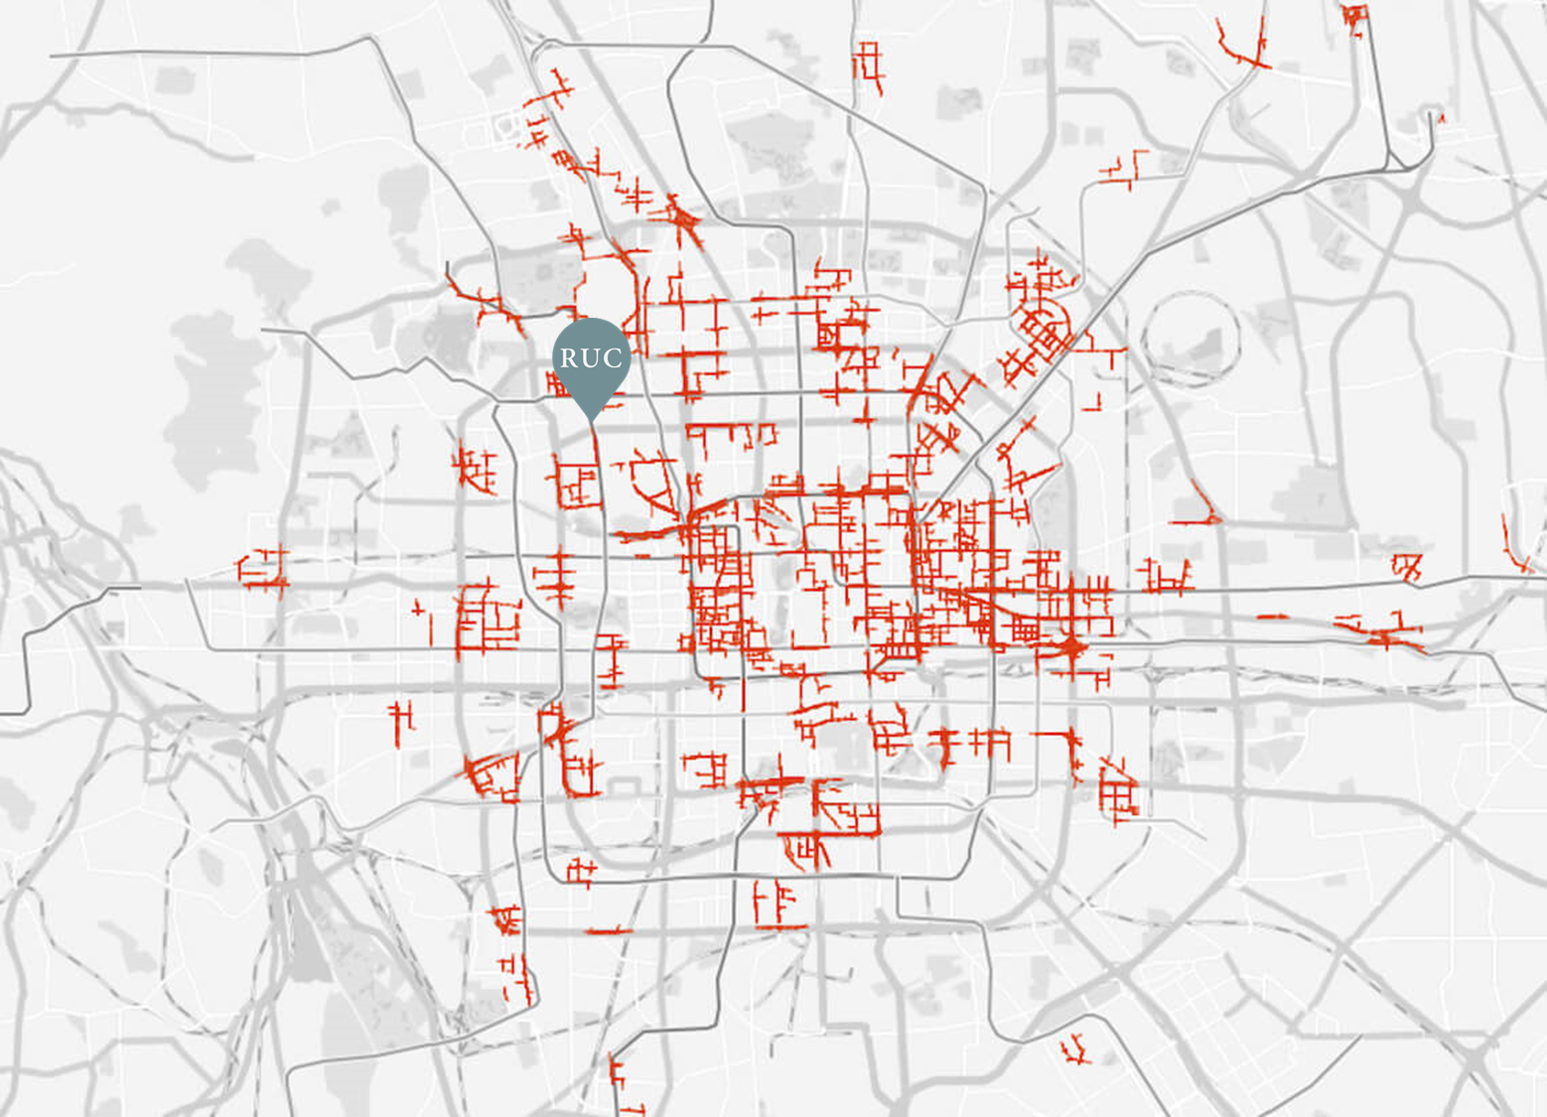
\includegraphics[width=0.5\textwidth]{image/road_map.png}
  \caption{Q-TRAFFIC数据集中路段分布图,标注出为人大东门}
  \label{fig1}
\end{figure}

为方便使用,公开数据中将速度处理为每15分钟的平均速度。Road Network数据集则记录了每天道路的道路编号,起始点的经纬度,道路宽度和长度、限速速度、车道数量等详细信息。Query数据集是通过百度地图收集到的,同时间内用户所有的地图查询记录,共计114,000,000条,包括查询时间,查询路线的终点和起点的经纬度,预计所用时间等信息。可以作为大规模交通预测时的辅助信息。




在本篇论文中我通过经纬度查询,匹配到距离中国人民大学(北纬39.9696, 东经116.3188)欧式距离最近的道路节点(如图\ref{fig1})。最终在Traffic Speed数据集中提取出从2017年4月1日到2017年5月1日,人民大学东门外主干道上每15分钟的车流平均速度,数据长度为$4\times24\times61=5856$。

\subsection{数据预处理}
\begin{figure}[htbp]
  \centering
  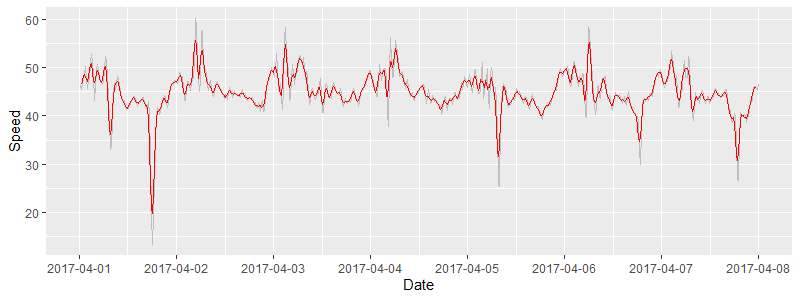
\includegraphics[width=0.8\textwidth]{image/filter.png}
  
  \caption{中国人民大学东门外主干道车流速度,以4月1日到4月7日这一周的数据为例。灰线为原序列(每15分钟)的平均速度,红线为处理后的每小时日均速度}
\label{fig2}
\end{figure}

原序列的数据为每15分钟一次,所以数据量和数据波动都较大,给后期建模带来了很大的开销。为了方便后期建模,更好的挖掘长期规律,我将原序列处理成每小时的平均速度,数据总长度减小为$5856/4=1464$,平滑结果如图\ref{fig2}所示。同时,因为本次研究的目的时提取车流速度在每日和每周的变化规律,将数据处理为每小时的平均速度也是合理的。

为了评估模型的效果,我将数据按照3:1的比例划分为训练集和测试集两个部分。将前六周的数据(总长为1008)作为训练数据,最后一周的数据(总长为336)作为测试数据。

\subsection{模型建立}
\subsubsection{平稳性检验与周期性探究}
探究平稳性和周期性是建立MSARIMA和DSHW模型的基础。平稳性可以通过直接观察时序图、观察acf自相关图等方式进行判断。对于车流速度数据,由于时间节点较多,我这里先画出前一个月的序列。
\begin{figure}[htbp]
  \centering
  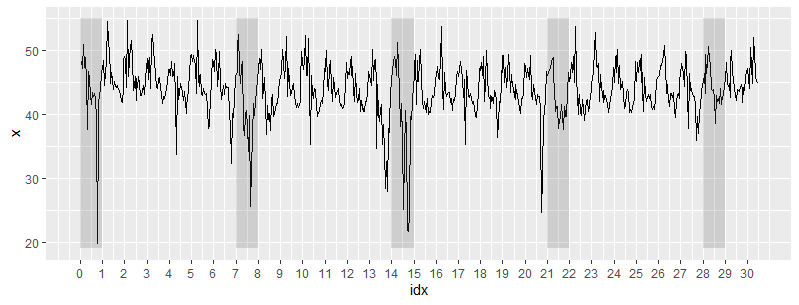
\includegraphics[width=\textwidth]{image/first_month.png}
  
  \caption{中国人民大学东门外主干道车流速度前一个月数据。可以发现较为明显的日周期性和周周期性}
\label{fig3}
\end{figure}  

通过前一个月的时序图(如图\ref{fig3}),我们可以发现如下规律:
\begin{enumerate}[(1)]
    \item 序列具有较明显的日周期性,每天都会在大致相同的时间点出现波峰和波谷,大多数波峰波谷高度相似。
    \item 序列有较明显的周周期性。序列开始的时间为四月一日星期六。从时序图上来看,从第一天开始,大致每隔七天,也就是在每周的周末都会产生一次相比往日更大的波谷。
    \item 除过周期性之外,这两个月的的车流速度大致都在固定的数值上下波动,说明没有明显的趋势特征。
\end{enumerate}

为了验证判断,同时我也画出了车速数据的acf图,延迟最大值设为三周的长度$24\times7\times3$(如图\ref{fig4})。通过自相关图,我们发现序列确实有多重周期性。一方面,acf图的走势大致为正弦函数,在每延迟k天处都出现波峰。另一方面以7天为周期,在延迟7、14、21天的位置,自相关系数达到的波峰比往日更高,说明路况数据具有一定的周周期性。

\begin{figure}[htbp]
  \centering
  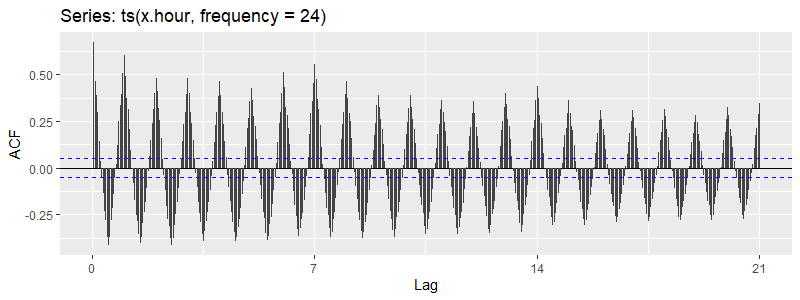
\includegraphics[width=\textwidth]{image/acf_1.png}
  \caption{原序列的acf图,延迟最大值设为$24\times7\times3$,以天为单位}
  \label{fig4}
\end{figure}  

\subsubsection{多周期ARIMA模型(MSARIMA)}

\textbf{消除周期性}

根据4.3.1的描述,可以将车流速度数据看作是具有$s_1=24,s_2=24\times7=168$的双周期序列,并且没有趋势特征。所以可以分别通过168步差分和24步差分,依次消除周周期和日周期性,将序列转化为平稳序列。

图\ref{fig5.1}和图\ref{fig5.2}是进行168步差分后的自相关系数图和偏自相关系数图。从acf图可以看出,序列的周期性已经被消除了很多。在横坐标等于7,14,21的地方acf图已经看不出来明显的突变,说明周周期性已经被基本消除了。但是从五天内的acf图来看,在短期的几天(第一天、第二天、第三天)仍然有较为明显的相关性,这说明日周期性仍然有很大一部分残留。同时,随着天数的增加,相关系数逐渐变小,这也说明了长时间的周期性(周周期性)已经被消除。

在已经消除周周期性的数据的基础上,再做24步差分,以消除日周期性。通过差分后的acf图(图\ref{fig5.3})可以看出,除了第一天acf骤降之外,其余部分没有明显的骤增或骤降,说明短期的日周期性也基本消除掉了。另外,经过ADF检验,所有的p值都小于0.05,差分后的序列显著平稳(见表\ref{tab:4})。

\begin{figure}[H]
\centering 
\subfigure[168步差分后的ACF图]{
\label{fig5.1}
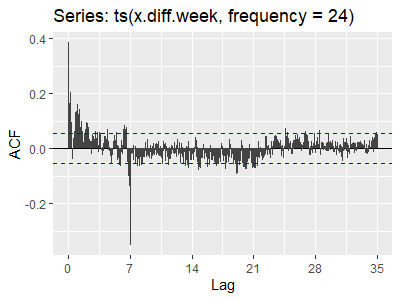
\includegraphics[width=0.45\textwidth]{image/x_week_acf.png}}
\subfigure[168步差分后的PACF图]{
\label{fig5.2}
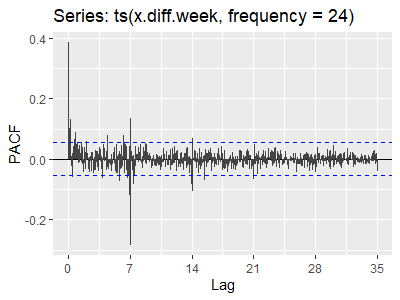
\includegraphics[width=0.45\textwidth]{image/x_week_pacf.png}}

\subfigure[24步差分后的ACF图]{
\label{fig5.3}
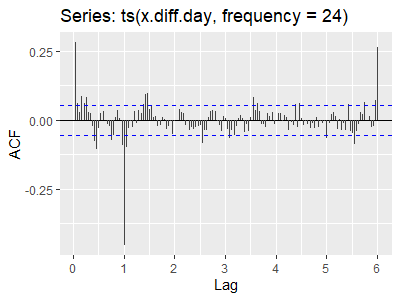
\includegraphics[width=0.45\textwidth]{image/x_day_acf.png}}
\subfigure[24步差分后的PACF图]{
\label{fig5.4}
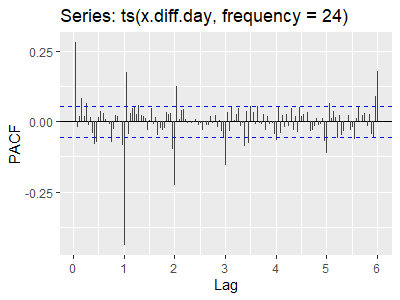
\includegraphics[width=0.45\textwidth]{image/x_day_pacf.png}}
\caption{Main name}
\label{Fig.main}
\end{figure}


\textbf{模型定阶}

根据3.1的介绍,对于双周期时间序列可以建立模型$\mathrm{ARIMA}(p,d,q)\times(P_1,D_1,Q_1)_{S_1}\times(P_2,D_2,Q_2)_{S_2}$。进一步还需要对模型定阶,也就是确定具体的$p,d,q,P_1,D_1,Q_1,P_2,D_2,Q_2$的值。

首先确立无周期性的短期相关模型部分。对于依次进行$24$步差分和$168$步差分之后的序列,观察其acf图(图\ref{fig5.3})和pacf图(图\ref{fig5.4}),发现在24阶以内自相关系数和偏自相关系数均不截尾,考虑用低阶的ARMA(1,1)来提取短期自相关信息。

对于日周期自相关特征,观察以延迟24阶、48阶等以周期长度为单位的自相关系数和偏自相关系数,发现自相关系数在除延迟24阶显著非0之外,以周期长度为单位的自相关系数都在两倍标准差以内,而偏自相关系数有一定的截尾特征但不明显,所以采用以24步为周期$ARIMA(0,1)_{24}$提取日周期的自相关信息

周周期的自相关特征可以通过只做了168步差分的序列的自相关系数和偏自相关系数判断。画出只消除周周期的序列的自相关图(图\ref{fig5.1})和偏自相关图(图\ref{fig5.2}),观察以延迟168阶、336阶等以168为单位的自相关系数和偏自相关系数,我们发现自相关系数在延迟168阶以后都落入了两倍标准差内,偏自相关系数也在延迟504阶后落入两倍标准差内,所以可以认为周周期的自相关特征是自相关系数截尾、偏自相关系数也截尾的,可以考虑用$ARMA(3,0)_{168}$提取周周期自相关特征。

最终确定,我们要拟合的模型是$\mathrm{ARIMA}(1,0,1)\times(0,0,1)_{24}\times(3,0,0)_{168}$

\textbf{参数估计}

在R软件中,forecast包中的msarima函数可以拟合多周期的ARIMA模型。利用ARIMA模型,可以得到参数的估计值如表\ref{tab:1}.

\begin{table}[!htbp]
\caption{ARIMA(1,0,1)(0,0,1)[24](3,0,0)[168]参数拟合结果}
\centering
\label{tab:1}
\setlength{\tabcolsep}{6mm}{
\begin{tabular}{cccc}
\hline
      & 1       & 24     & 168     \\ \hline
AR(1) & 0.6945  & -      & 0.2026  \\ 
AR(2) & -       & -      & 0.0214 \\
AR(3) & -       & -      & 0.7688  \\
MA(1) & -0.1794 & 0.3304 & - \\
\hline
\end{tabular}}
\end{table}

根据拟合输出结果,最终建立的模型为

\begin{equation}
\nabla_{24}\nabla_{168}x_t=\frac{(1-0.1794B)(1+0.3304B^{24})}{(1+0.6945B)(1+0.2026B^{168}+0.0214B^{336}+0.7688B^{504})}\varepsilon_t
\end{equation}

\textbf{ARCH模型}

通过建立多季节的ARIMA模型,原车流速度序列中的周期性已经基本被提取出来。为进一步判断模型是否已经提取出来原序列的全部信息,还需要对残差进行进一步检验。

通过残差图\ref{fig9.1},我们发现残差具有一定的集群效应,后半段比前半段变化更加剧烈。通过白噪声检验,绘制出p随延迟期数变化的变化情况,发现p在100以内呈现迅速减小的趋势(如图\ref{fig9.2})。通过拉格朗日乘子检验,发现p值非常小,残差具有显著的自相关性。通过比较拟合模型的系数显著性,最终选择ARCH(2)模型作为残差的拟合模型

最终,拟合的模型为

\begin{equation}
\left\{
\begin{aligned}
&\nabla_{24}\nabla_{168}x_t=\frac{(1-0.1794B)(1+0.3304B^{24})}{(1+0.6945B)(1+0.2026B^{168}+0.0214B^{336}+0.7688B^{504})}\varepsilon_t\\
&\varepsilon_t=\sqrt{h_t}e_t\\
&e_t=1.99520+0.49827\varepsilon_{t-1}^2+0.30873\varepsilon_{t-2}^2
\end{aligned}
\right.
\end{equation}

绘制条件异方差模型拟合图如下图(图\ref{fig6}),发现ARCH(2)模型可以较好的拟合出MSARIMA没有提取出的异方差信息。

\begin{figure}[H]
\centering  %图片全局居中
\subfigure[ARCH模型拟合结果与原残差对比]{
\label{fig6.1}
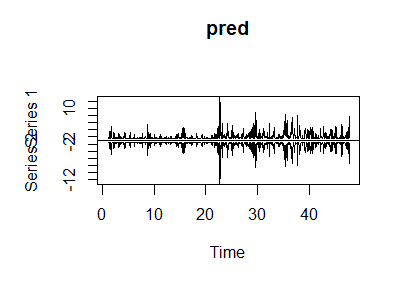
\includegraphics[width=0.45\textwidth]{image/arch1.png}}
\subfigure[ARCH模型置信区间]{
\label{fig6.2}
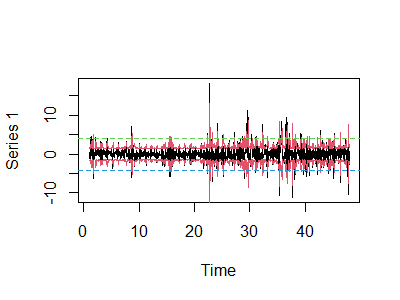
\includegraphics[width=0.45\textwidth]{image/arch2.png}}
\caption{ARCH模型的结果}
\label{fig6}
\end{figure}

\subsubsection{双季节Holt-winters指数平滑模型(DSHW)}
如前文介绍的,乘积形式的DSHW指数平滑模型如下:
\begin{equation}
\begin{aligned}
a_t&=\alpha(x_t/s_tr_t)+(1-\alpha)(a_{t-1}+b_{t-1})\\
b_t&=\beta(a_t-a_{t-\Pi_1})+(1-\beta)b_{t-1}\\
s_t&=\gamma(x_t/a_tr_t)+(1-\gamma)s_{t-\pi_1}\\
r_t&=\delta(x_t/a_ts_t)+(1-\delta)r_{t-\pi_1}\\
\end{aligned}
\end{equation}

对于人民大学东门外主干道车流的每小时平均速度数据来说,设置日周期长度$\pi_1=24$,周周期长度$\pi_2=24\times7=168$。可以设计算法,通过最小化预测均方误差,找到系数$\alpha,\beta,\gamma,\delta$的估计值,拟合车流速度数据。在R软件中`forecast`包提供了`dshw()`函数,可以按照这样的思路拟合模型。得到的拟合结果如表\ref{tab:2}。

\begin{table}[!htbp]
\caption{DSHW模型参数拟合结果}
\centering
\label{tab:2}
\setlength{\tabcolsep}{4mm}{
\begin{tabular}{cccccc}
\hline
\textbf{参数}  & $\alpha$  & $\beta$   & $\gamma$  & $\delta$  & $\phi$    \\ \hline
\textbf{估计值} & 0.0133 & 0.0020 & 0.0230 & 0.2652 & 0.3504 \\ \hline
\end{tabular}}
\end{table}

观察模型拟合结果,参数$\alpha,\gamma,\delta$,均比较大,说明车流速度数据确实有比较明显的日周期和周周期性。

同时我们发现趋势部分参数$\beta=0.002$明显小于其他参数。这说明虽然从直观来看,在2017年的四五两个月车流速度在固定数值上下波动,但是由潜在的缓慢递增趋势。造成这一结果的原因可能时潜在的月周期变化,也可能是模型的过度拟合。但由于数据量的限制,我们不能挖掘出月周期变化规律,真实的原因还需要更多数据量的支持。

\subsection{模型评估}
\subsubsection{预测准确率}
为了检验模型的效果,首先比较两个模型在预测新数据上的准确率。实际实验中,我将前6周的数据作为训练集,后2周的数据作为测试集,用在训练集上拟合的模型预测后两周的车流速度。RMSE、EC和MAPE是三个衡量预测准确率的指标,其定义如下


\begin{equation}
RMSE=\sqrt{\frac{1}{L}\sum\limits_{i=1}^{L}(y_i-\hat{y}_i)^2}
\end{equation}
\begin{equation}
EC=1-\frac{\sqrt{\sum\limits_{i=1}^{L}(y_i-\hat{y}_i)^2}}{\sqrt{\sum\limits_{i=1}^{L}y_i^2}+\sqrt{\sum\limits_{i=1}^{L}\hat{y}_i^2}}
\end{equation}

\begin{equation}
MAPE=\frac{1}{L} \sum\limits_{i=1}^L \frac{yi - \hat{y}_i}{yi}\times100
\end{equation}

其中$L$表示向后预测的期数,$y_i$表示真实值,$\hat{y}_i$表示模型的预测值。在这里$L=24\times7\times2=336$。两个模型的预测结果和真实值如图\ref{fig.7}和图\ref{fig.8}所示。从表\ref{tab:3}看,MSARIMA模型的RMSE、EC和MAPE分别3.511727,0.958342和6.156587;DSHW法分别是2.507141、0.974319和3.862283。可以看出,从预测的角度来看,DSHW方法的预测准确程度略高于ARIMA模型。结合预测图来看DSHW方法对于峰值拟合的更好。

\begin{table}[htbp]
\caption{两种模型预测准确率比较}
\centering
\label{tab:3}
\setlength{\tabcolsep}{5mm}{
\begin{tabular}{cccc}
\hline
        & RMSE     & MAPE     & EI       \\ \hline
MSARIMA & 3.511727 & 6.156587 & 0.958342 \\
DSHW      & \textbf{2.507141} & \textbf{3.862283} & \textbf{0.974319} \\ \hline
\end{tabular}}
\end{table}

\begin{figure}[H]
\centering  %图片全局居中
\subfigure[MSARIMA]{
\label{fig7.1}
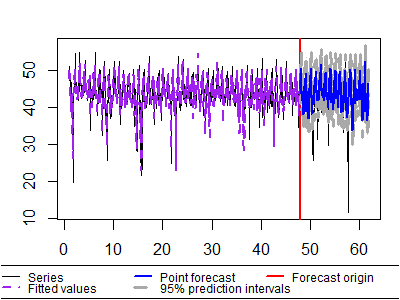
\includegraphics[width=0.45\textwidth]{image/predict2.png}}
\subfigure[DSHW]{
\label{fig7.2}
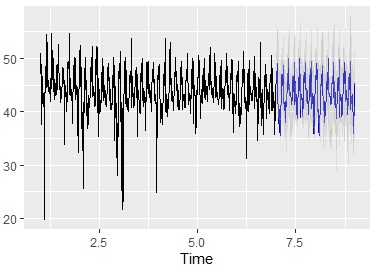
\includegraphics[width=0.45\textwidth]{image/predict_ds.png}}
\caption{MSARIMA模型和DSHW模型的预测结果}
\label{fig.7}
\end{figure}

\begin{figure}[htbp]
  \centering
  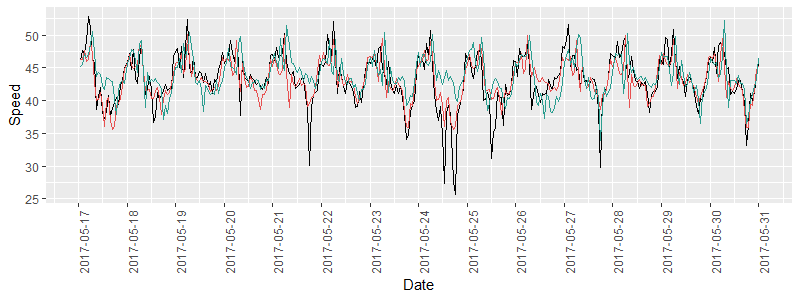
\includegraphics[width=\textwidth]{image/predict.png}
  \caption{预测结果比较。红色为DSHW方法的预测值,绿色为MSARIMA模型的预测值,黑色为真实值}
  \label{fig.8}
\end{figure}  

\subsubsection{平稳性检验}
通常来说在建立ARMA模型之前需要判断建模序列的平稳性。对于原数据来说,从acf图已经能明显看出序列不平稳。但是,对于经过24步差分和168步差分之后的序列需要再进行一次平稳性检验,确保后续建模的合理性。在这里,我才用ADF检验作为序列平稳性的判断。由于原序列周期长度较长,所以延迟阶数的选择较长。这里依次选择从1到168的阶数,做出ADF检验的p值表格\ref{tab:4}。所有的检验的p值都很小,说明差分后的序列显著平稳,MSARIMA的后续建模是合理的。

\begin{table}[H]
\caption{ADF检验p值}
\centering
\label{tab:4}
\begin{tabular}{cccccccccccc}
\hline
延迟期数 & 6 &  12 &  18 &  24 &  30 &  36 &  42 &  48 &  54 &  60 &  66 \\ \hline
p值 & \textless{}0.01 &  \textless{}0.01 &  \textless{}0.01 &  \textless{}0.01 &  \textless{}0.01 &  \textless{}0.01 &  \textless{}0.01 &  \textless{}0.01 &  \textless{}0.01 &  \textless{}0.01 &  0.012204 \\ \hline
\end{tabular}
\end{table}

\subsubsection{残差白噪声检验}
通过检测残差序列是否满足纯随机性质,可以看出模型对原序列信息提取得是否充分。纯随机性可以通过acf图看,如果自相关系数越小,说明序列的随机性就越明显。纯随机性也可以构造LB统计量(Box Ljung)来看。根据LB统计量近似服从卡方分布,检验自相关系数是否都显著为0。

通过自相关图(\ref{fig9})来看,通过两种模型的提取,残差序列的自相关系数都很小。并且长期来看,残差序列没有时间趋势,没有发生周期性的波动。这说明两个模型对于原序列的规律性信息,尤其是周期性信息,提取的都比较完整,具有很好的拟合效果。

\begin{figure}[htbp]
\centering  %图片全局居中
\subfigure[]{
\label{fig9.1}
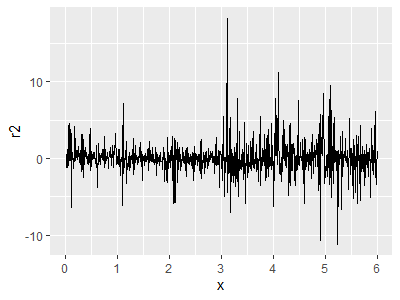
\includegraphics[width=0.20\textwidth]{image/res_2.png}}
\subfigure[]{
\label{fig9.2}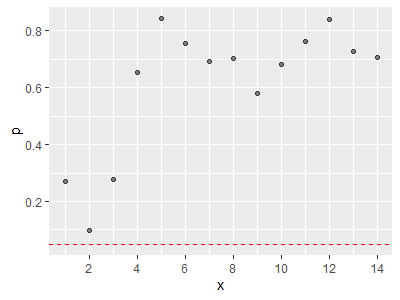
\includegraphics[width=0.20\textwidth]{image/res_2_p.png}}
\subfigure[]{
\label{fig9.3}
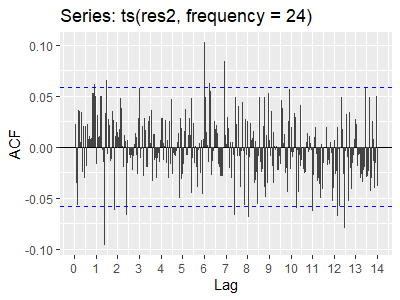
\includegraphics[width=0.20\textwidth]{image/res2_acf.png}}
\subfigure[]{
\label{fig9.4}
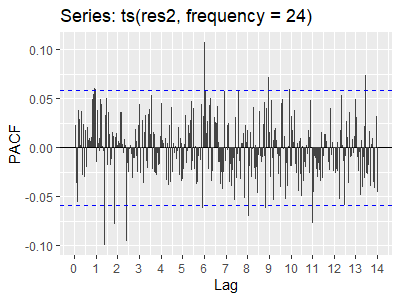
\includegraphics[width=0.20\textwidth]{image/res2_pacf.png}}

\subfigure[]{
\label{fig9.5}
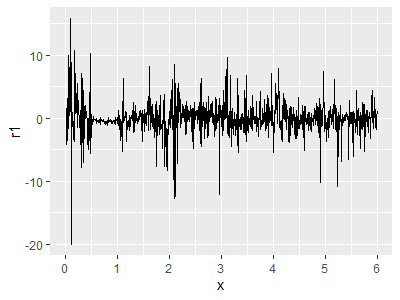
\includegraphics[width=0.20\textwidth]{image/res_ds.png}}
\subfigure[]{
\label{fig9.6}
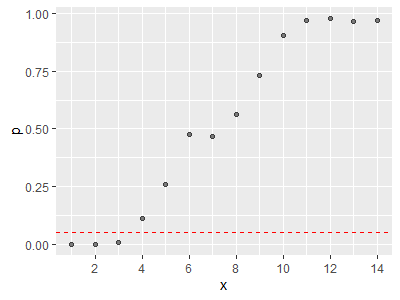
\includegraphics[width=0.20\textwidth]{image/res_ds_p.png}}
\subfigure[]{
\label{fig9.7}
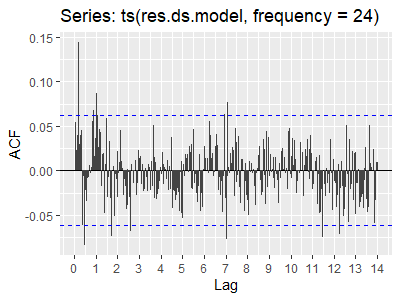
\includegraphics[width=0.20\textwidth]{image/res_ds_acf.png}}
\subfigure[]{
\label{fig9.8}
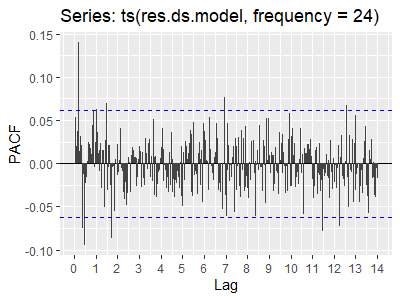
\includegraphics[width=0.20\textwidth]{image/res_ds_pacf.png}}
\caption{残差检验结果,第一行为MSARIMA模型,第二行为DSHW模型。从左到右依次是残差图、Box检验的p值和延迟阶数的关系图、自相关图和偏自相关图。}
\label{fig9}
\end{figure}


为了严格检验残差的自相关系数是否显著为0,我进一步构造了LB统计量进行假设检验。由于周期长度较长,检验时将延迟阶数选择为两倍的最大周期长度,也就是$2*24*7$,并依次绘制出如下p值随延迟阶数变化的图。在图中我们发现ARIMA模型的残差在延迟阶数为40左右p值降到了0.05以下,DSHW模型的残差在延迟阶数小于80时,很大一部分的p值都小于0.05,说明残差在短期内有一定的非随机性,原序列中还存在一些信息的残留。在4.3.2中,我通过建立ARCH模型进一步拟合残差中的自相关性和异方差性,通过拟合图[],残差的拟合效果很好,自相关性基本消除了。但是由于MSARIMA-ARCH模型有些复杂,现有的R包只适用单季节的SARIMA-ARCH模型,MSARIMA-ARCH所以没有用来实际预测。


\section{总结与讨论}
这次研究的重点在于对于多周期序列的建模。人大东门外主干道车流数据具有很明显的日周期和周周期性,我以这个数据为例,主要采用了MSARIMA模型和DSHW指数平滑模型两种方法拟合数据,提取出数据中的周期性信息,并用来预测之后两周的车流平均速度。从预测结果上看,两个模型都达到了不错的效果,DSHW模型的预测准确率略高于MASRIMA模型。

但是两个模型的残差都具有不同程度的信息残留。与MSARIMA模型相比,DSHW模型残留的更多。对于MSARIMA模型,我通过建立ARCH(2)模型提取出了残差中的自相关和异方差信息,拟合效果很好。但是由于最后的模型较为复杂,且没有直接的R包支持,MSARIMA-ARCH模型没能用来做预测。以后的工作可以尝试从这一点出发,建立R代码实现多季节的MSARIMA-ARCH模型和MSARIMA-GARCH模型的拟合和预测工作。

\nocite{*}
\bibliography{wpref}

\end{document}
